\documentclass{beamer}
\usepackage[fontsize=17pt]{fontsize}
\usepackage{graphicx}
\usepackage{tikz}
\usepackage{svg}
\usepackage[polish]{babel}
\usepackage{booktabs}
\usepackage{colortbl}
\usepackage{multirow}
\usepackage{amssymb}
\graphicspath{ {./images/} {../../latex/tex/img/} }
\usetheme{Warsaw}

%Information to be included in the title page:
\title{\large Porównanie wydajności i możliwości \\ współczesnych silników gier komputerowych}
\author{inż. Krzysztof Rudnicki}
\institute{
    \textbf{Promotor:} dr inż. Michał Chwesiuk \\[0.3em]
    Wydział Elektroniki i Technik Informacyjnych \\
    Politechnika Warszawska
}
\date{\scriptsize 10 marca 2026}

\setbeamertemplate{footline}[frame number]{}
\beamertemplatenavigationsymbolsempty
\setbeamertemplate{headline}{}

\begin{document}

%==============================================================================
% TITLE
%==============================================================================
\begin{frame}
  \vspace{-0.5cm}
  \maketitle
\end{frame}

%==============================================================================
% TABLE OF CONTENTS
%==============================================================================
\begin{frame}
\frametitle{Plan prezentacji}
\tableofcontents
\end{frame}

%==============================================================================
% SECTION 1: MOTIVATION AND GOALS
%==============================================================================
\section{Cel i zakres pracy}

\begin{frame}
  \frametitle{Motywacja}
  \begin{itemize}
    \item Rynek gier zdominowany przez dwa silniki:
    \begin{itemize}
      \item \textbf{Unity} -- prawie 25\,000 gier na Steam
      \item \textbf{Unreal Engine} -- ponad 7\,500 gier na Steam
    \end{itemize}
    \item Brak systematycznych badań porównawczych
  \end{itemize}
\end{frame}

\begin{frame}
  \frametitle{Cel pracy}
  \begin{enumerate}
    \item Testy wydajności z~NVIDIA Nsight Systems
    \item Implementacja identycznej gry w obu silnikach
    \item Analiza porównawcza funkcjonalności
    \item Wywiady z~8 deweloperami gier
  \end{enumerate}
\end{frame}

\begin{frame}
  \frametitle{Hipoteza}
  \vspace{1cm}
  \centering
  \large
  Unity osiągnie lepszą wydajność w~grze 2D \emph{bullet hell} dzięki natywnemu wsparciu dla grafiki 2D.
\end{frame}

%==============================================================================
% SECTION 2: METHODOLOGY
%==============================================================================
\section{Metodologia}

% SKRYPT: Wybór gatunku -- bullet hell
% Uzasadnienie:
% - Setki/tysiące pocisków na ekranie
% - Test zarządzania pamięcią (GC vs ręczne)
% - Intensywne wykrywanie kolizji
% - Skalowalność obciążenia
% - Prosta koncepcja -> fokus na wydajność
{
  \setbeamercolor{footline}{fg=white}
  \usebackgroundtemplate{
    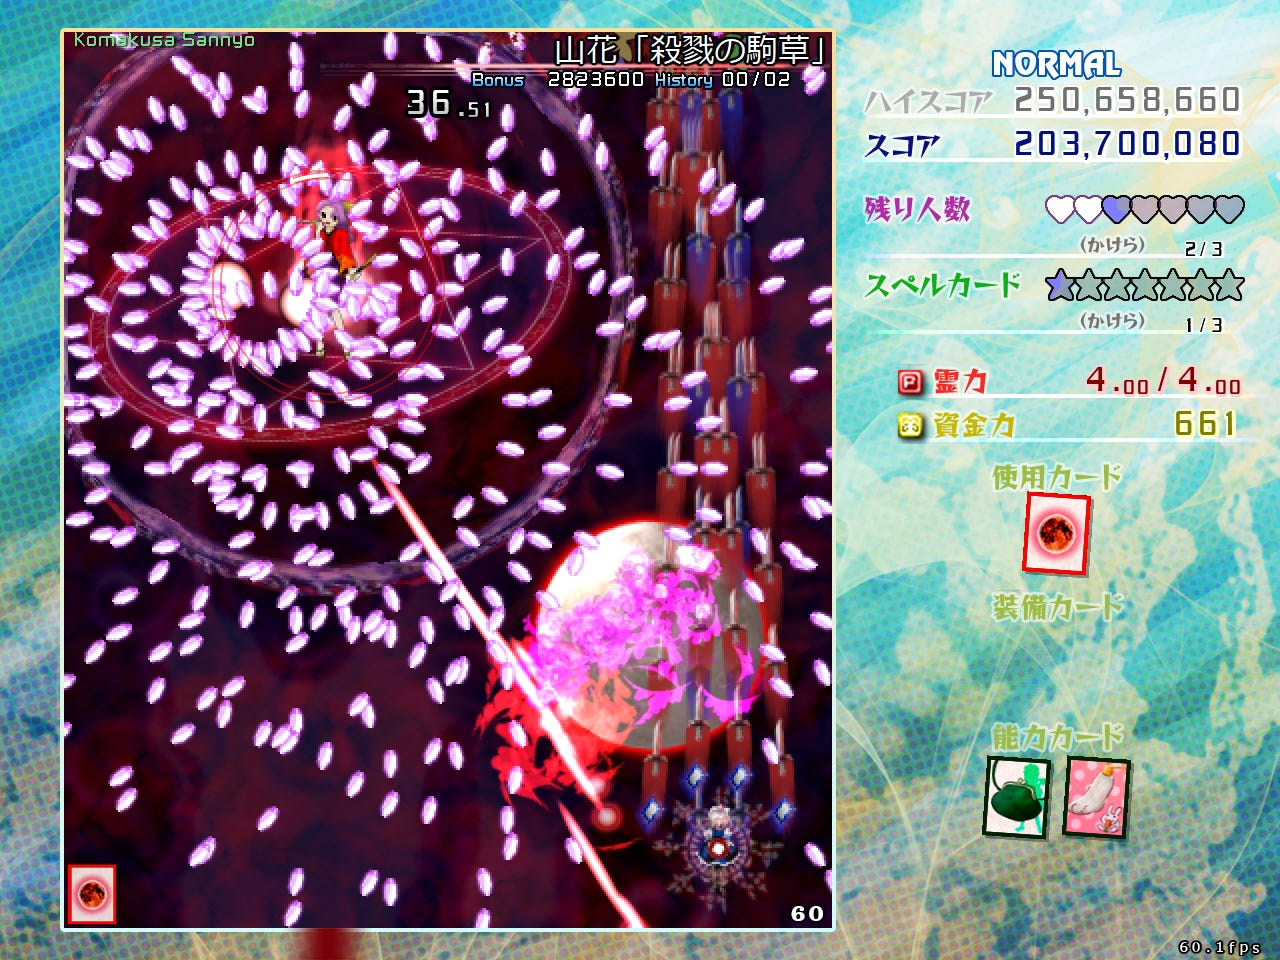
\includegraphics[width=\paperwidth, height=\paperheight]{touhou.jpg}}
  \begin{frame}
  \end{frame}
}

\begin{frame}
  \frametitle{Parametry gry testowej}
  \begin{itemize}
    \item Czas rozgrywki: \textbf{90 sekund}
    \item 3 typy przeciwników z różnymi wzorcami strzelania
    \item Eskalacja trudności w 3 fazach
    \item Limit: 200 jednoczesnych przeciwników
    \item Interwał spawnu: 0,25s $\rightarrow$ 0,08s
  \end{itemize}
\end{frame}

\begin{frame}
  \frametitle{Środowisko testowe}
  \begin{table}
    \centering
    \footnotesize
    \renewcommand{\arraystretch}{1.1}
    \begin{tabular}{@{}ll@{}}
      \toprule
      CPU & AMD Ryzen 9 7900X3D \\
      GPU & NVIDIA RTX 3090 (24 GB) \\
      RAM & 32 GB \\
      OS & Arch Linux \\
      Unity & 6.0 LTS \\
      Unreal & 5.5.3 \\
      Profiler & NVIDIA Nsight Systems 2025.5.2 \\
      \bottomrule
    \end{tabular}
  \end{table}
\end{frame}

%==============================================================================
% SECTION 3: IMPLEMENTATION
%==============================================================================
\section{Implementacja}

\begin{frame}
  \frametitle{Implementacja -- Unity}
  \begin{itemize}
    \item Język: \textbf{C\#}
    \item Natywny tryb 2D
    \item \texttt{Rigidbody2D}, \texttt{Collider2D}
    \item Object pooling: \texttt{SetActive()}
    \item Hot reload
    \item Instalacja: $\sim$30 min
  \end{itemize}
\end{frame}

{
  \setbeamercolor{footline}{fg=white}
  \usebackgroundtemplate{
    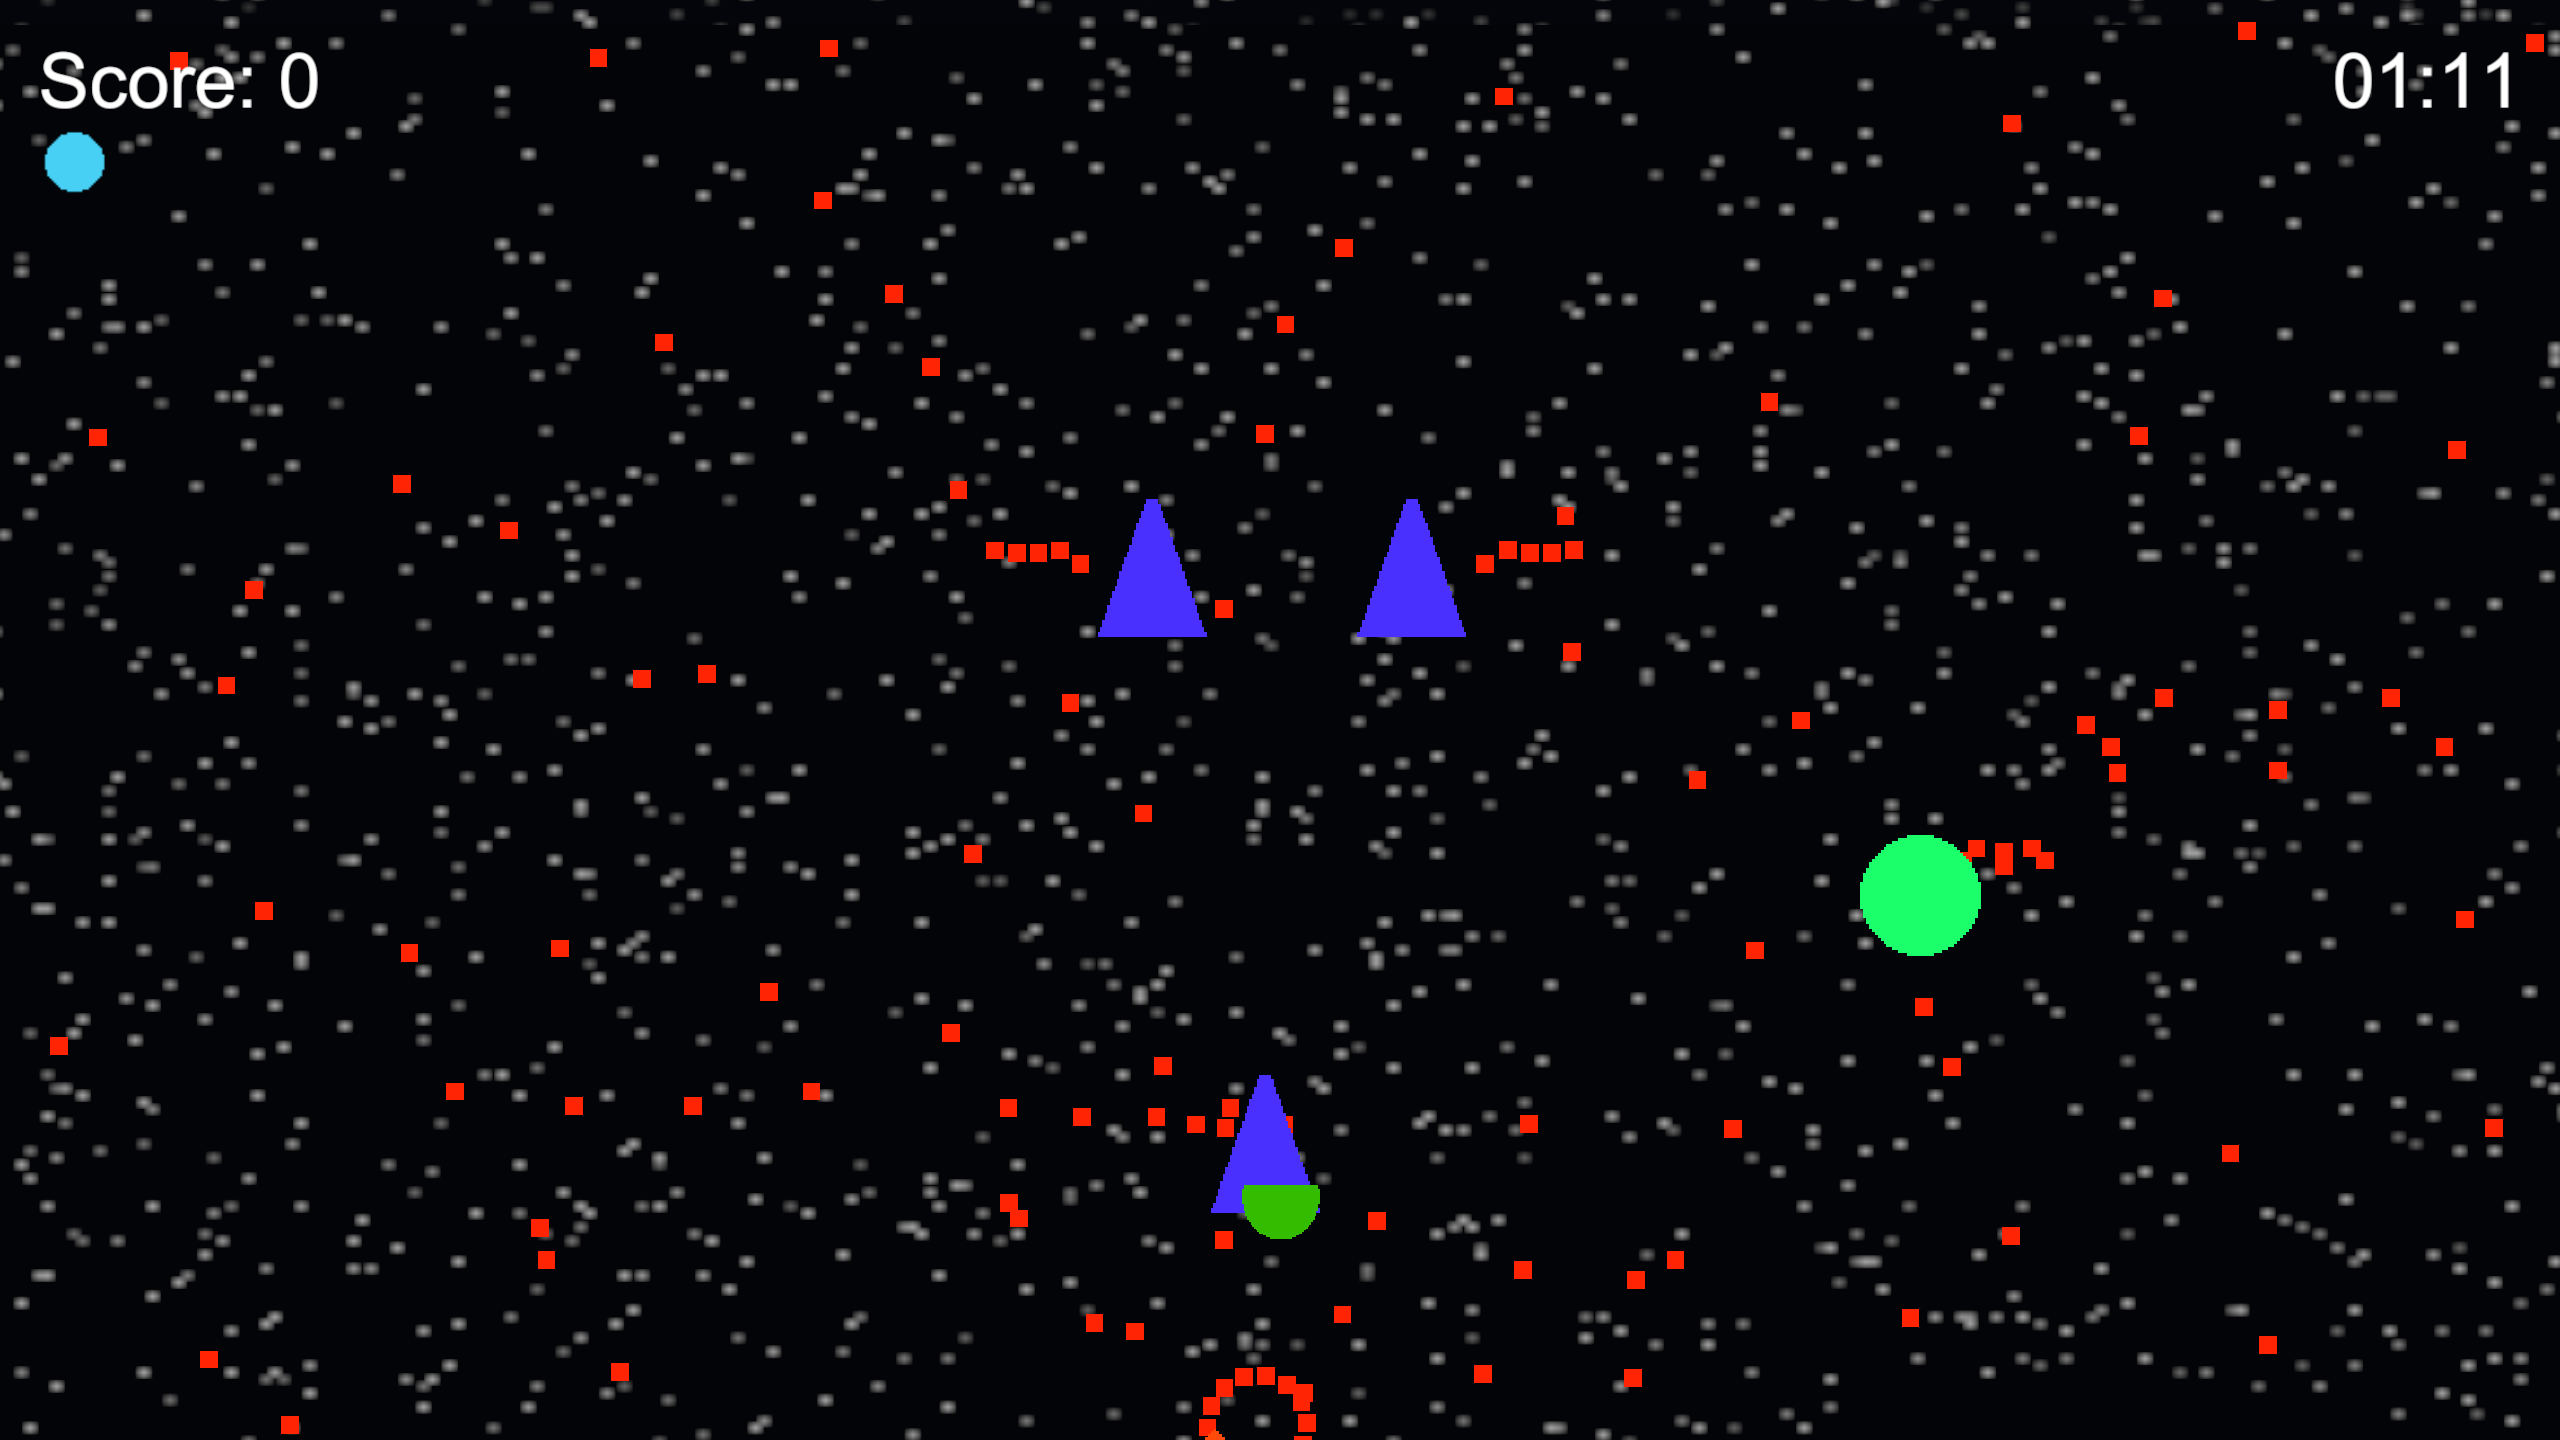
\includegraphics[width=\paperwidth, height=\paperheight]{unity_game.png}}
  \begin{frame}
  \end{frame}
}

\begin{frame}
  \frametitle{Implementacja -- Unreal Engine}
  \begin{itemize}
    \item Język: \textbf{C++} / Blueprinty
    \item ,,Fałszywe 2D'' w środowisku 3D
    \item Object pooling -- 3 metody:
    \begin{itemize}
      \scriptsize
      \item \texttt{SetActorHiddenInGame}
      \item \texttt{SetActorEnableCollision}
      \item \texttt{SetActorTickEnabled}
    \end{itemize}
    \item Instalacja: $\sim$2--4h (Linux)
  \end{itemize}
\end{frame}

{
  \setbeamercolor{footline}{fg=white}
  \usebackgroundtemplate{
    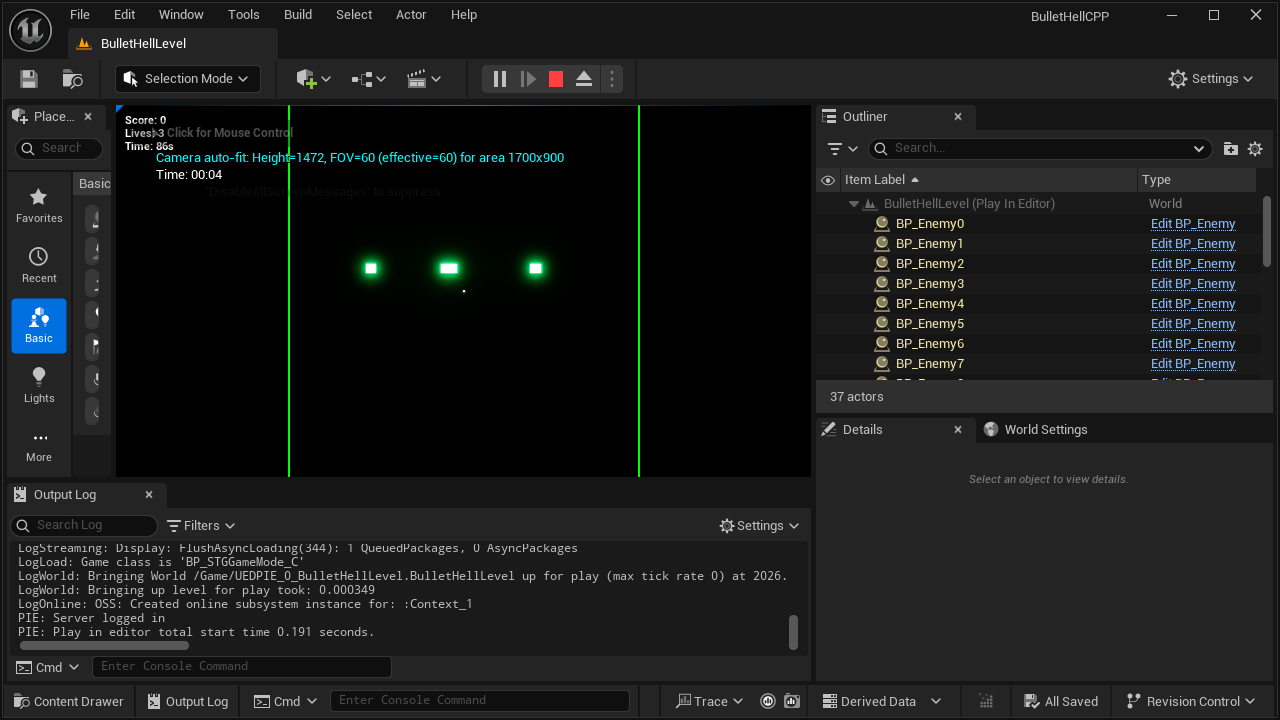
\includegraphics[width=\paperwidth, height=\paperheight]{unreal_game_view.png}}
  \begin{frame}
  \end{frame}
}

\begin{frame}
  \frametitle{Porównanie doświadczeń implementacyjnych}
  \begin{table}
    \centering
    \small
    \begin{tabular}{lcc}
      \toprule
      \textbf{Aspekt} & \textbf{Unity} & \textbf{Unreal} \\
      \midrule
      Instalacja (Linux) & $\sim$30 min & $\sim$2--4 h \\
      Natywne 2D & Tak & Nie \\
      Język & C\# & C++ \\
      Próg wejścia & Niski & Średni/Wysoki \\
      Czas kompilacji & Szybki & Wolny \\
      Object pooling & Prosty & Złożony \\
      Hot reload & Tak & Ograniczony \\
      \bottomrule
    \end{tabular}
  \end{table}
\end{frame}

%==============================================================================
% SECTION 4: PROFILING TOOL
%==============================================================================
\section{Narzędzie profilowania}

% SKRYPT: Dlaczego nie wbudowane profilery?
% Wbudowane profilery silników są nieporównywalne:
% - Różna definicja metryk
% - Różny narzut profilowania
% - Różne formaty wyjściowe
\begin{frame}
  \frametitle{Dlaczego NVIDIA Nsight Systems?}
  \begin{itemize}
    \item NVIDIA Nsight -- niezależne narzędzie:
    \begin{itemize}
      \item Zunifikowane metryki sprzętowe
      \item Analiza na poziomie Vulkan API
      \item Minimalny narzut (poziom sterownika)
      \item Spójny format dla obu silników
    \end{itemize}
  \end{itemize}
\end{frame}

{
  \setbeamercolor{footline}{fg=white}
  \usebackgroundtemplate{
    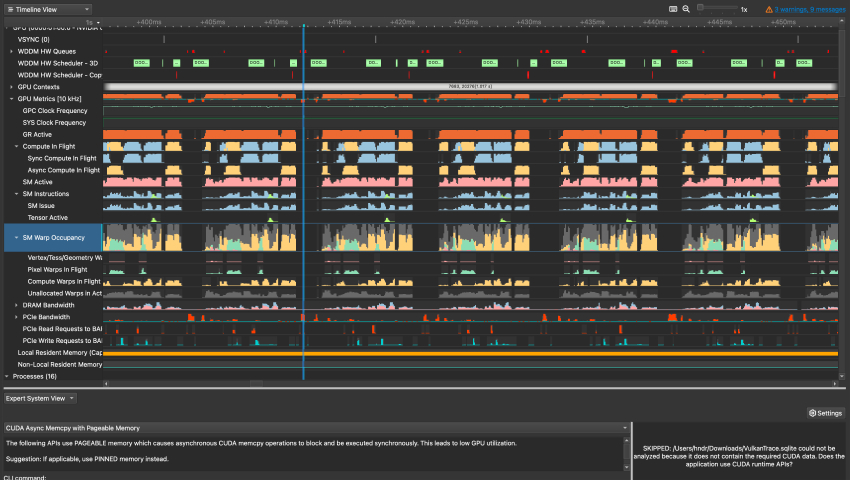
\includegraphics[width=\paperwidth, height=\paperheight]{nvida_nsighty.jpg}}
  \begin{frame}
  \end{frame}
}

%==============================================================================
% SECTION 5: PERFORMANCE RESULTS
%==============================================================================
\section{Wyniki testów wydajności}

\begin{frame}
  \frametitle{Unity -- wydajność klatek}
  \begin{table}
    \centering
    \footnotesize
    \renewcommand{\arraystretch}{1.1}
    \begin{tabular}{@{}lr@{}}
      \toprule
      Czas testu & 94,16 s \\
      Wyrenderowane klatki & 13\,556 \\
      Średni FPS & 143,96 (V-Sync: 144 Hz) \\
      Mediana czasu klatki & 6,94 ms \\
      99. percentyl (1\% low) & 7,58 ms (132 FPS) \\
      Klatki w 5--10 ms & \textbf{98,24\%} \\
      IQR czasu klatki & 0,08 ms \\
      \bottomrule
    \end{tabular}
  \end{table}
\end{frame}

\begin{frame}
  \frametitle{Unity -- architektura renderowania}
  \small
  \begin{itemize}
    \item \textbf{Prosty potok}: 2 wywołania \texttt{vkQueueSubmit}/klatkę
    \item \texttt{vkWaitForFences} -- \textbf{95,2\%} czasu Vulkan API
    \begin{itemize}
      \item CPU czeka na GPU $\rightarrow$ scenariusz \textbf{GPU-bound}
    \end{itemize}
    \item Łącznie $\sim$218\,815 wywołań Vulkan API
    \item Tylko \textbf{3 potoki graficzne} w~całym teście
    \item Wykorzystanie GPU: \textbf{$\sim$23\%} (ograniczone V-Sync)
  \end{itemize}
\end{frame}

\begin{frame}
  \frametitle{Unreal Engine -- wydajność klatek}
  \begin{table}
    \centering
    \small
    \begin{tabular}{lrrr}
      \toprule
      \textbf{Metryka} & \textbf{Faza 1} & \textbf{Faza 2} & \textbf{Faza 3} \\
      \midrule
      Średni FPS & 332 & 339 & 162  \\
      GPU Active & 91\% & 91\% & 50\% \\
      vkQueueSubmit & 166\,918 & 186\,589 & 74\,393 \\
      Submit/klatkę & 16,2 & 16,2 & 16,2  \\
      \bottomrule
    \end{tabular}
  \end{table}
  \vspace{0.3cm}
  \begin{itemize}
    \item Spadek o~\textbf{ponad 50\%} między fazami 1--2 a~fazą 3
    \item Brak V-Sync -- pełne wykorzystanie GPU
  \end{itemize}
\end{frame}

\begin{frame}
  \frametitle{Unreal Engine -- architektura renderowania}
  \small
  \begin{itemize}
    \item \textbf{Złożony potok}: 16 wywołań \texttt{vkQueueSubmit}/klatkę
    \item Tworzenie potoków: \textbf{47--72\%} czasu Vulkan API
    \begin{itemize}
      \item $\sim$1000 potoków na fazę (vs 3 w Unity!)
    \end{itemize}
    \item Łącznie $\sim$\textbf{32 mln} wywołań Vulkan API
    \item $\sim$\textbf{9 mln} wywołań synchronizacji OS
    \item Intensywne użycie compute shaderów (culling, post-proc.)
  \end{itemize}
\end{frame}

\begin{frame}
  \frametitle{Porównanie kluczowych wyników}
  \begin{table}
    \centering
    \small
    \begin{tabular}{lrr}
      \toprule
      \textbf{Metryka} & \textbf{Unity} & \textbf{Unreal} \\
      \midrule
      Wykorzystanie GPU & 23\% & 91\% / 50\% \\
      Wywołania Vulkan API & $\sim$0,5 mln & $\sim$32 mln \\
      Wywołania sync. OS & 29\,383 & $\sim$9 mln \\
      Potoki graficzne & 3 & $\sim$2\,400 \\
      Submit/klatkę & 2 & 16 \\
      \bottomrule
    \end{tabular}
  \end{table}
\end{frame}

\begin{frame}
  \frametitle{Interpretacja -- Unity}
  \begin{block}{Unity}
    \begin{itemize}
      \item Prosty, dwuetapowy potok -- wydajny dla gier 2D
      \item Stabilne czasy klatek (98,24\% w 5--10 ms)
      \item Niewykorzystany potencjał GPU (V-Sync: 23\%)
    \end{itemize}
  \end{block}
\end{frame}

\begin{frame}
  \frametitle{Interpretacja -- Unreal Engine}
  \begin{block}{Unreal Engine}
    \begin{itemize}
      \item Złożony, wieloetapowy potok -- narzut dla prostych scen
      \item Ciągła rekompilacja potoków (dynamiczna optymalizacja)
      \item Pełne wykorzystanie GPU ($\sim$91\%)
      \item Spadek wydajności przy dużym obciążeniu ($>$50\%)
    \end{itemize}
  \end{block}
\end{frame}

%==============================================================================
% SECTION 6: INTERVIEWS
%==============================================================================
\section{Wywiady z~deweloperami}

\begin{frame}
  \frametitle{Wywiady -- najważniejsze wnioski (1/2)}
  8 respondentów (1--10 lat doświadczenia):
  \vspace{0.2cm}
  \begin{itemize}
    \item \textbf{Próg wejścia}: Unity niższy, Unreal wyższy
    \item \textbf{Dokumentacja}: Unity lepsza (przykłady kodu); Unreal -- ,,szkieletowa''
    \item \textbf{Blueprinty}: Ułatwiają współpracę z~nietechnicznymi, ale problemy z~Git
  \end{itemize}
\end{frame}

\begin{frame}
  \frametitle{Wywiady -- najważniejsze wnioski (2/2)}
  \begin{itemize}
    \item \textbf{Architektura}: Unreal wymusza porządek; Unity -- elastyczny
    \item \textbf{C\# vs C++}: C\# łatwiejszy; C++ w~Unreal ,,niestandardowy''
    \item \textbf{Materiały}: Unity przewaga ilościowa
  \end{itemize}
\end{frame}

%==============================================================================
% SECTION 7: CONCLUSIONS
%==============================================================================
\section{Wnioski}

\begin{frame}
  \frametitle{Weryfikacja hipotezy}
  \textit{,,Unity osiągnie lepszą wydajność w~grze bullet hell~\ldots''}
  \vspace{0.5cm}

  \begin{itemize}
    \item Prostsza architektura renderowania
    \item Stabilniejsze czasy klatek
    \item Łatwiejszy proces implementacji (60\% czasu)
    \item Natywne wsparcie 2D
  \end{itemize}
\end{frame}

\begin{frame}
  \frametitle{Rekomendacje}
  \begin{table}
    \centering
    \footnotesize
    \renewcommand{\arraystretch}{1.1}
    \begin{tabular}{@{}lll@{}}
      \toprule
      \textbf{Projekt} & \textbf{Silnik} & \textbf{Powód} \\
      \midrule
      2D indie & Unity & Natywne 2D \\
      Mobilna & Unity & Optymalizacja \\
      Prototyp & Unity & Szybkie iteracje \\
      3D AAA & Unreal & Nanite, Lumen \\
      VR high-end & Unreal & Oświetlenie \\
      Zespół mieszany & Unreal & Blueprinty \\
      \bottomrule
    \end{tabular}
  \end{table}
\end{frame}

\begin{frame}
  \frametitle{Wkład pracy}
  \begin{enumerate}
    \item \textbf{Zunifikowana metodyka pomiaru} -- \\ Nsight Systems jako niezależne narzędzie
    \item \textbf{Analiza Vulkan API} -- \\ 32 mln wywołań (Unreal) vs 0,5 mln (Unity)
    \item \textbf{Triangulacja metod} -- \\ testy + wywiady + implementacja
    \item \textbf{Praktyczne rekomendacje} -- \\ macierz wyboru silnika
  \end{enumerate}
\end{frame}

\begin{frame}
  \frametitle{Ograniczenia}
  \begin{itemize}
    \item Jeden gatunek gry (bullet hell)
    \item Pojedyncza konfiguracja sprzętowa (high-end)
    \item 8 wywiadów (badanie eksploracyjne)
  \end{itemize}
\end{frame}

\begin{frame}
  \frametitle{Dalsze badania}
  \begin{itemize}
    \item Testy dla RPG, RTS, puzzle
    \item Różne platformy (mobile, konsole, low-end PC)
    \item Automatyczny framework benchmarkowy
    \item Badanie długoterminowe (2--3 lata)
  \end{itemize}
\end{frame}

\begin{frame}
  \frametitle{}
  \vspace{2cm}
  \centering
  {\Large Dziękuję za uwagę}
  \vspace{1cm}

  {\normalsize Pytania?}
\end{frame}

\end{document}